\documentclass{report}


%%%%%%%%%%%%%%%%%%
%   Liste des packages utilisés  %
%%%%%%%%%%%%%%%%%%

% (oui y'en a 95% qui sont inutiles ^^)

\usepackage{amssymb}
\usepackage{array}
\usepackage{hyperref}
\usepackage{booktabs}
\usepackage{multirow}
\usepackage{float}
\usepackage{lmodern} %Pack de police
\usepackage{color}
\usepackage[dvipsnames]{xcolor}
\usepackage{graphicx}
\usepackage[utf8x]{inputenc}
\usepackage[T1]{fontenc}
\usepackage{natbib}
\usepackage[francais]{babel}
\usepackage{caption}
\usepackage{listings}
\usepackage{booktabs}
\usepackage[top=2cm, bottom=2cm,left=2cm, right=2cm]{geometry}
\usepackage{blindtext}
\usepackage{setspace}
\usepackage{graphicx}
\usepackage{titlesec, blindtext, color} % titres spéciaux + couleur pour les chapter

% on transforme les chapters en juste le numéro suivi du titre, avec un barre grisse
\definecolor{gray75}{gray}{0.75}
\newcommand{\hsp}{\hspace{20pt}}
\titleformat{\chapter}[hang]{\Huge\bfseries}{\thechapter\hsp\textcolor{gray75}{|}\hsp}{0pt}{\Huge\bfseries}


%\titleformat{\chapter}[display]
%	{\normalfont\huge\bfseries}{}{0pt}{\Huge}
\renewcommand\thesubsection{\arabic{subsection}}

\titlespacing*{\subsection}{0pt}{2.0ex plus 1ex minus .2ex}{0.5ex plus .2ex}
\titlespacing*{\subsubsection}{0pt}{1.0ex plus 1ex minus .2ex}{0.5ex plus .2ex}

\begin{document}


%%%%%%%%%%%
%  Page de garde  %
%%%%%%%%%%%
\begin{titlepage}
	\begin{center}
	
		\begin{spacing}{1.5}
			Projet Picross\\
			\vspace*{\fill}
		\end{spacing}
		
		\begin{spacing}{2.5}
			\textbf{\Huge Application de création et d'aide à la résolution de puzzle \textit{picross}}\\[0.5cm]
			\textbf{\huge Cahier d'analyse et conception} \\
			\vspace*{\fill}
			\textit{Étudiants :}
		\end{spacing}

		\begin{spacing}{1.15}
			\large
			\textsc{Brinon} Baptiste\\
			\textsc{Brocherieux} Thibault\\
			\textsc{Cohen} Mehdi\\
			\textsc{Debonne} Valentin\\
			\textsc{Lardy} Anthony\\
			\textsc{Mottier} Emeric\\
			\textsc{Pastouret} Gilles\\
			\textsc{Pelloin} Valentin\\
			\vspace*{\fill}
			\textbf{Groupe n°2} \\
			\textnormal{\large Licence Informatique\\ Le Mans Université\\ \today}
		\end{spacing}
		
	\end{center}
\end{titlepage}


%%%%%%%%%%
%    Sommaire    %
%%%%%%%%%%
\renewcommand{\contentsname}{Sommaire}
\tableofcontents


\chapter{Présentation}

	\section{Introduction}

		Dans le cadre de l'unité d'enseignement "Génie logiciel 2" de la Licence d'informatique de Le Mans Université, les étudiants de troisième année sont amenés à travailler sur un projet de développement d'une application. \\
		Ce document permet de présenter les solutions au cahier des charges, ainsi que l'architecture du programme demandé. Celui-ci est divisé en plusieurs parties : l’architecture du jeu, la gestion d'une partie, l'aide à la résolution du picross, %la gestion des statistiques du joueur (scores, niveaux débloqués, …)% ainsi que l’interface graphique. Ce document décrit aussi l'utilisation du temps qui nous est imparti. 

	
 	\section{Objectif de l'application}		
		Nous devons réaliser un jeu de type picross (aussi appelé \textit{nonogramme}, logigramme ou \textit{hanjie}) permettant à un utilisateur de résoudre des grilles et de l'aider dans sa réalisation.
		
	\section{Outils}
		
		Afin de réaliser notre application de \textit{picross}, nous utilisons plusieurs outils.
LaTeX est utilisé pour rédiger et mettre en forme les différents livrables avant de les convertir en format PDF.
\textit{Git} et \textit{GitHub} permettent le partage d'informations et la mise en commun du code ainsi que les livrables associés. Nous nous servons de \textit{Discord} afin de communiquer au sein du groupe, partager nos idées, nos informations et notre travail.
Pour concevoir les différents diagrammes UML, nous avons recours au logiciel \textit{Astah} et au site internet \textit{Tom's Planner}.
Afin de créer les maquettes du logiciel (disponibles en Annexe) permettant d’avoir un rendu de la future interface graphique, nous avons utilisé le logiciel \textit{Balsamiq}.
Pour simplifier la vérification de la qualité du code produit, nous utilisons Code Climate (maintenabilité) ainsi que Travis CI(compilation et tests).
Le language de programmation Ruby est utilisé pour programmer le logiciel, incluant une documentation générée par \textit{RDoc}. L’utilisation des bibliothèques de \textit{GTK} sera utilisé pour la réalisation des interfaces graphiques.

		
\chapter{Conception générale}

    \section{Diagramme de Gantt détaillé}
    
    \begin{figure}[H]
	\caption{Diagramme de \textit{Gant détaillé}}
	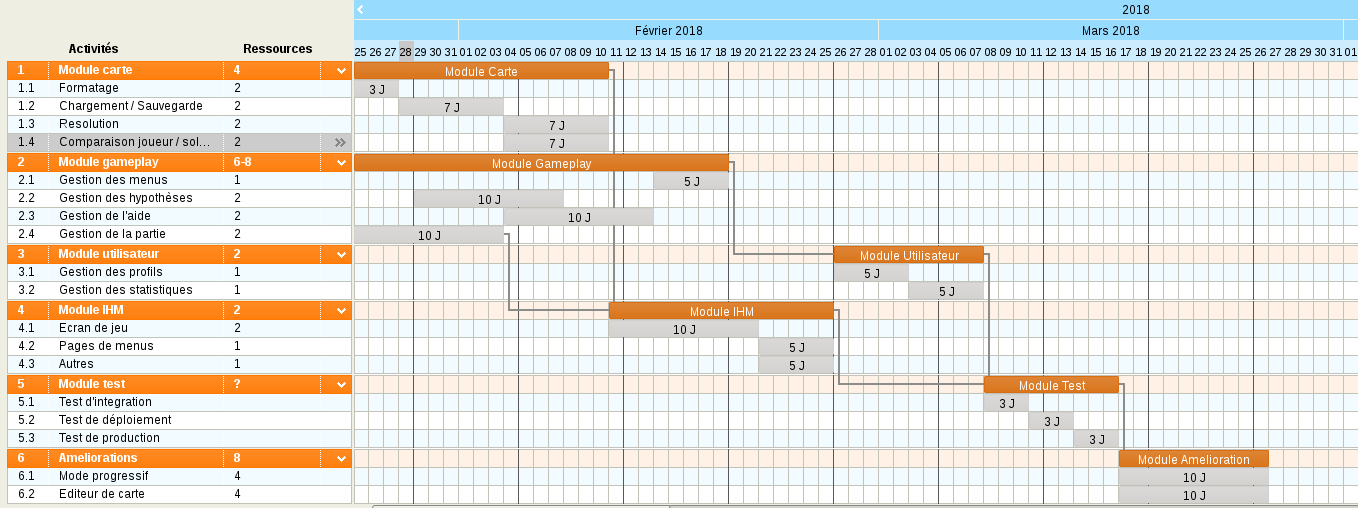
\includegraphics[width=17cm]{ganttDetaille.png}
    \end{figure}
   
     À travers ce diagramme de Gantt, nous observons l'organisation du projet sur les trois mois à venir. Le projet se découpe en plusieurs modules : carte, gameplay, utilisateur, IHM, test et améliorations.
    Chaque module a une durée de vie, nous lui accordons un temps de travail et un certain nombre de personnes, les modules sont également divisés en différentes étapes ce qui correspond aux fonctionnalités de l'application. Les modules sont imbriqués les uns dans les autres, c'est-à-dire que certains dépendent d'autres modules. Sans les modules gameplay et carte réalisés, le module IHM ne peut être réalisé. 

   \section{Besoins fonctionnels}
   
    En plus de la génération et de la gestion d'une partie, le programme doit contenir les fonctionnalités suivantes:

 \setcounter{secnumdepth}{5}
 
 	\subsection{Proposer une aide adaptée au niveau de difficulté}
 		\subsubsection{Appel d'aide sanctionné, sauf cas contraire}
 				L'utilisateur pour utiliser l'aide à tout moment en échange d'une perte de temps, sauf si celui-ci dispose d'une aide gratuite.
		\subsubsection{Niveau didacticiel}
				L'utilisateur peut accéder à un chapitre dédié à l'apprentissage des règles du picross et du fonctionnement du logiciel.

    \subsection{Utilisation d'un chronomètre}
			\subsubsection{Génération de scores en fin de partie}
				A la fin de la partie, un nombre d'étoiles est attribué au joueur en fonction du temps écoulé.
			\subsubsection{Mise en pause possible}
				A n'importe quel moment de la partie, le joueur peut la mettre en pause. Elle est alors masquée
	
	\subsection{Hypothèses}
		\subsubsection{Créer une hypothèse}
			Durant la partie, le joueur peut créer une nouvelle hypothèse en cliquant sur le bouton associé. Les cases colorées seront alors d'une couleur différente.
		\subsubsection{Valider une hypothèse}
			Lorsque l'hypothèse s'avère juste, l'utilisateur peut choisir de la valider. Les cases colorées deviennent alors noires et l'hypothèse disparait de celles en cours.
		\subsubsection{Annuler une hypothèse}
			Lorsque l'hypothèse est fausse, l'utilisateur pour l'annuler. Les cases colorées suite à la création de l'hypothèse sont alors blanchies.
		
	\subsection{Système de sauvegardes}
		\subsubsection{Sauvegardes effectuées automatiquement}
			A chaque modification de la grille, une nouvelle sauvegarde est effectuée automatiquement, sauvegardant aussi la valeur du chronomètre.
		\subsubsection{Chargement automatique des sauvegardes au redémarrage de la partie}
			Lorsque le joueur relance une partie qu'il n'avait pas terminée, le chronomètre reprends là ou il était arrêté, et la grille est affichée là ou l'avait laissée le joueur
			
	\subsection{Statistiques}
		\subsubsection{Mise à jour automatique des statistiques}
			A chaque fin de partie, les statistiques sont mises à jour en fonction du score que le joueur à réalisé lors de cette partie.	
		\subsubsection{Consultables dans le menu associé}
			Dans les menus, le joueur peut afficher ses statistiques.
			
	\subsection{Interface Homme Machine}
		\subsubsection{Grilles en noir et blanc, avec couleurs réservées aux hypothèses.}
			Les cases sont blanches, et peuvent etre colorées en noir. Lors d'une hypothèse, la couleur peut varier.
		\subsubsection{Jouable uniquement au clavier, ou uniquement à la souris, ou avec les 2}
			Le joueur peut jouer avec les périphériques qu'il désire, que ce soit seulement au clavier, seulement à la souris, ou les deux en même temps.
		\subsubsection{Mise en valeur des chiffres associés aux cases cochées}
			Quand le joueur colorie des cases, le programme identifie de quel chiffre il s'agit et le met en valeur de façon à faciliter la lisibilité de la grille.
		\subsubsection{Affichage de la quantité de cases colorées en une selection (selection multiple)}
			Quand l'utilisateur selectionne plusieurs cases en une fois, un petit chiffre à coté de la souris (ou de la case sur laquelle se trouve le curseur s'il joue au clavier) indique le nombre de cases actuellement concernées.
		
   \section{Diagramme de cas d'utilisations}
      
    \begin{figure}[H]
	\caption{Diagramme de \textit{Cas d’utilisation}}
	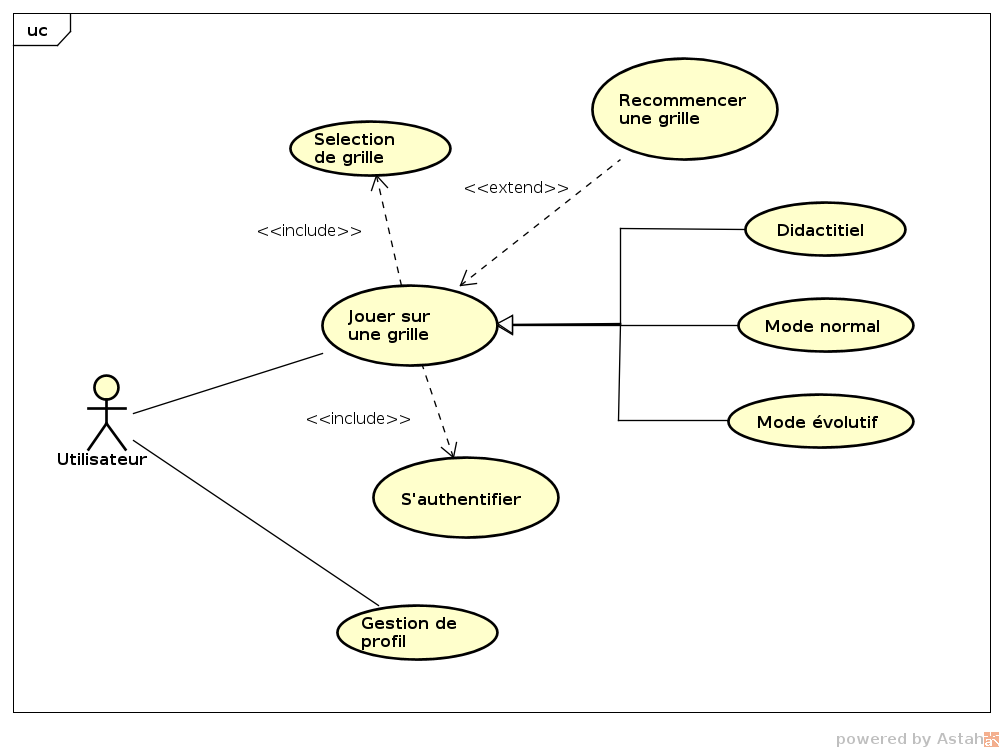
\includegraphics[width=17cm]{../UML/UseCase_diagram/UseCase1.png}
    \end{figure}
    
      %Description des cas d'utilisation

%% Reformuler
	Le but de l'utilisateur est de jouer sur une grille de \textit{picross}.
Pour cela, il doit avoir un profil. Il peut donc en créer un nouveau s'il en a envie, ou s'authentifier à un profil déjà existant.
	Le joueur doit ensuite sélectionner une grille à l'aide du menu. Il a le choix entre trois types de jeu :
	\begin{itemize}
	\item Le didacticiel, permettant d'apprendre les règles du jeu. 
	\item Le mode classique, permettant de jouer sur plusieurs grilles de tailles et difficultés variables.
	\item Le mode évolutif, agrandissant la taille de la grille au fur et à mesure que le joueur résoudra celle-ci.
	\end{itemize}
	À tout moment, celui-ci peut utiliser l'aide intégrée au jeu pour se débloquer. Il peut aussi choisir de recommencer la grille s'il le souhaite.

      
	\section{Mode classique}
		Dans le mode classique, le joueur a accès à plusieurs fonctionnalités. Il doit tout d'abord choisir un chapitre débloqué puis une grille. Ensuite, quand il se trouve en partie, il peut tout d'abord interagir avec la grille en cochant une case afin de se repérer dans les cases qui ne doivent pas être coloriées ou en coloriant une case. Il peut également enlever une coche ou une couleur d'une case s'il s'aperçoit qu'il s'est trompé. Il peut aussi sélectionner un groupe de cases à colorier, cocher ou vider. \\
		Au niveau de l'interface, l'utilisateur peut, à l'aide de boutons, réinitialiser la grille s'il souhaite repartir de zéro ou la valider s'il pense l'avoir finie. S'il la réussit, il sera renvoyé dans le chapitre en cours. Il peut également utiliser différentes aides (en cliquant sur un bouton) qui diffèrent par la clarté de l'indice, leur coût et leur pénalité. Enfin, l'utilisateur peut quitter la partie quand il le souhaite, la grille est sauvegardée automatiquement.
	
	\section{Mode evolutif}
	
	Lors d'une partie en mode évolutif, le joueur choisit une des grilles du mode. Chaque grille choisie a une taille fixe de 5x5 (cases). Pour résoudre cette grille, il a accès aux mêmes fonctionnalités qu'une partie classique soit interagir avec la grille et avec l'interface. \\
Une fois la grille réussie, celle-ci évolue en une grille plus grande (10x10) tout en gardant le coin supérieur gauche identique à la grille 5x5 réalisée par l'utilisateur (voir exemple en Annexe). Après cela, le joueur doit remplir la grille 10x10 en ayant les mêmes fonctionnalités que précédemment puis la grille évolue une nouvelle fois en 15x15 et ainsi de suite jusqu'à atteindre la taille maximale de 25x25. Une fois la grille 25x25 réussie, le joueur gagne la partie et est renvoyé sur le choix de la grille.
	
	% schéma exemple partie évolutive
	
	\section{Didacticiel}
	
	Une partie en mode didacticiel est une partie guidée afin que l'utilisateur comprenne la logique de résolution d'une partie de \textit{picross}. Les mouvements de celui-ci sont donc restreint aux coups (cocher ou colorier) que lui dit de jouer l'application.
	
	\section{erreurs}
	
		E1: Selection d'un chapitre non-déverouillé
			Peut arriver lors de la selection d'un chapitre
			Traitement: accés bloqué au chapitre et mesage rappellant le nombre d'étoiles manquante pour y accéder.
		E2: Arret de la partie en cours
			Peut arriver en cours de partie
			Traitement: lors du redemarrage de la partie, affichage d'un avertissement (partie quittée de façon non conventionnelle) et reprise au dernier point de sauvegarde.
			
  \section{Aides}

  L'utilisateur possède un nombre d'aides gratuites quand il commence à jouer et peut en récupérer en terminant un certain nombre de grille. Quand il est en jeu, il peut les utiliser afin de se débloquer sans pénalité de temps. S'il ne possède plus d'aides gratuites, alors il peut continuer d'utiliser l'aide, mais celle-ci aura un coût (en temps) proportionnel à la difficulté du picross qui sera appliqué à chaque utilisation. La difficulté influence aussi le type d'aide appliqué:
    \begin{itemize}
    \item En mode facile : coloriage de toute une ligne ou colonne
    \item En mode normal : coloriage d'une case correcte 
    \item En mode difficile : indication d'une ligne ou colonne où se trouve une case correcte non coloriée
    \end{itemize}


  \section{IHM}
  
  Les maquettes de l'interface sont accessibles en Annexe.
  
  
			
\chapter{Conception détaillé}

    \section{Diagramme de classe}
    
    \begin{figure}[H]
	\caption{Diagramme de \textit{Classes}}
	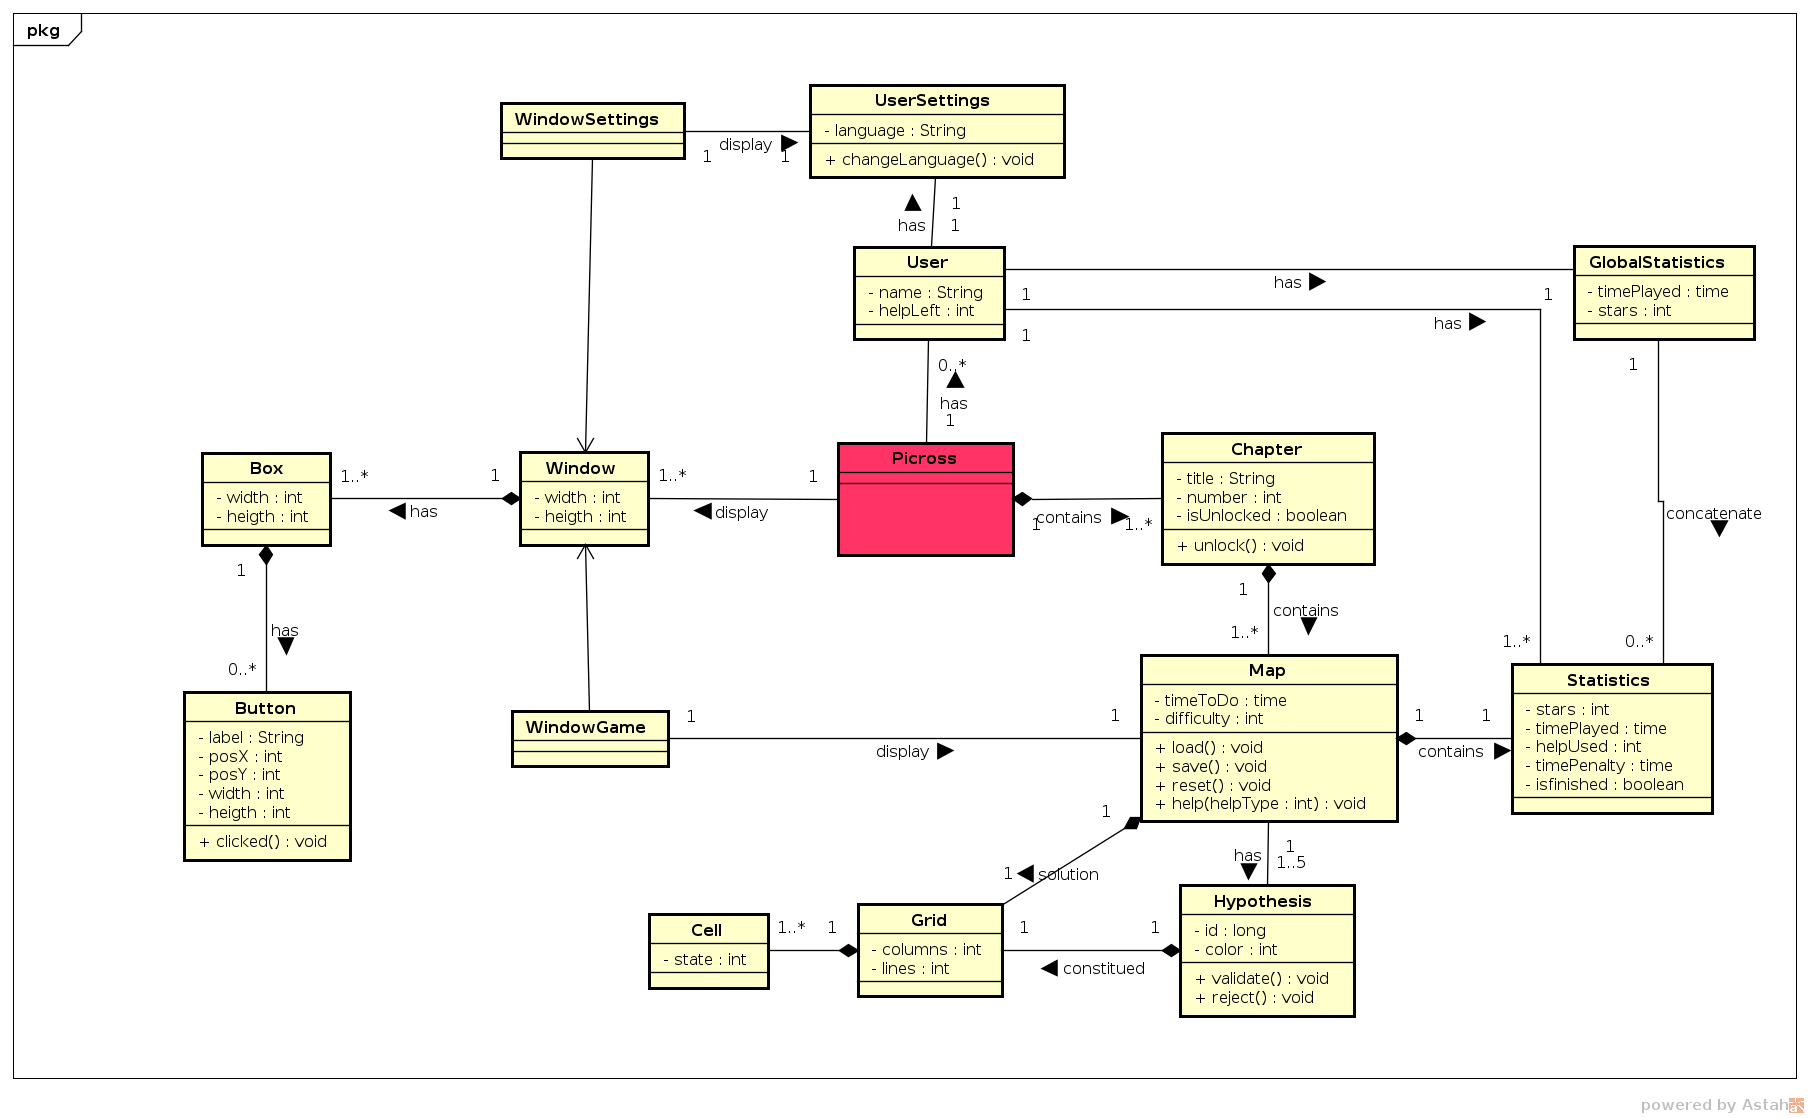
\includegraphics[width=17cm]{../UML/Class_diagram/DiagrammeClasse.png}
    \end{figure}
    
    	
	Le diagramme de classe ci-dessus présente les différentes classes que nous allons implémenter afin de programmer notre application. Nous avons tout d’abord la classe \textit{picross} qui est la racine permettant de rassembler toutes les autres classes et qui représente l’ensemble du jeu. Cette classe est liée à 3 modules principaux : l’Interface Homme-Machine, les données utilisateur, ainsi que le système de jeu.

	L’IHM commence par la classe Window correspondant à la fenêtre de l’application et possédant une taille définie et modifiable. Cette fenêtre contient plusieurs objets de classe Box possédant chacune une taille définie et représentant les différentes parties graphiques de la fenêtre (la grille, le chronomètre, l’affichage des informations, etc). Chacune de ces boîtes peut contenir des objets de classe Button correspondant aux boutons nécessaires à l’interaction entre l’utilisateur et le logiciel (valider la grille, retourner au menu, etc).

	Les données de l’utilisateur sont rassemblées dans la classe User possédant un pseudo, le nombre d’aides auxquelles il a le droit, et des données séparées en deux parties. La première correspondant aux différents paramètres du logiciel comme la langue utilisée ou la taille de la fenêtre (classe \textit{WindowSetting}) et modélisée grâce à la classe \textit{UserSettings}. La deuxième est liée aux statistiques  générales de l’utilisateur (classe \textit{GlobalStatistics}) comme le temps joué ou le nombre total d’étoiles ainsi que les statistiques liées à chaque grille finie par le joueur (classe \textit{Statistics}) comme le nombre d’étoiles reçues, le temps mis à la finir ainsi que le nombre d’aides utilisées.

 	Le système de jeu est rassemblé dans la classe \textit{Chapter} possédant un titre et un numéro ainsi qu’un booléen indiquant si ce chapitre est verrouillé ou non. Chaque chapitre est composé de plusieurs grilles représentées dans le diagramme par la classe \textit{Map} possédant une difficulté ainsi que le temps de base à réaliser la grille permettant ensuite de calculer le nombre d’étoiles obtenues par le joueur en fonction de son temps. Chacun de ses objets Map est capable de réaliser plusieurs actions comme s’initialiser, sauvegarder ou se réinitialiser. Lors d’une partie sur une grille, l’utilisateur peut utiliser le mode hypothèse représenté par la classe \textit{Hypothesis} composé d’un numéro et d’une couleur. Chacune de ses hypothèses est composée d’une sauvegarde de la grille (classe \textit{Grid}) avec l’état de chaque case (colorié, non colorié, croix) représenté par la classe \textit{Cell}.


\chapter{Annexes}

		\section{Exemple partie évolutive}
	
		Ci-joint sont présent des exemples de grilles évolutives, c'est-à-dire de grilles qui s'agrandissent au fil de la partie.
		Deux exemples de grilles sont disponibles sous forme de gif animé aux liens suivants :
		 \begin{itemize}
    		 \item \url{https://picross.vlntn.pw/Documents/Images/cat.gif}
   	   	 \item \url{https://picross.vlntn.pw/Documents/Images/mouse.gif}
		 \end{itemize}
		
		Le premier gif est également disponible sous format d'un ensemble d'images :
	
		\begin{figure}[H]
	       	 	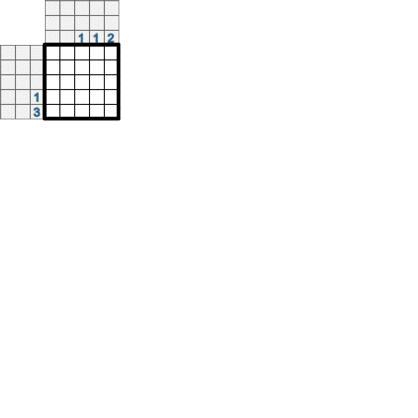
\includegraphics[width=5cm]{../Images/cat/cat1.png}
			\hspace{1cm}
          		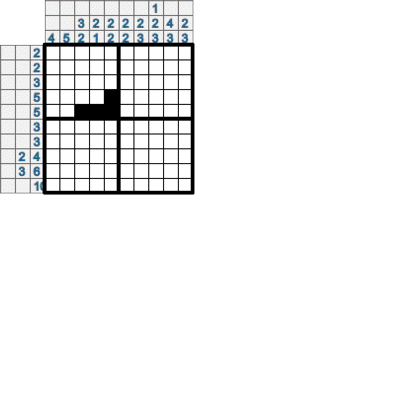
\includegraphics[width=5cm]{../Images/cat/cat2.png}
			\hspace{1cm}
			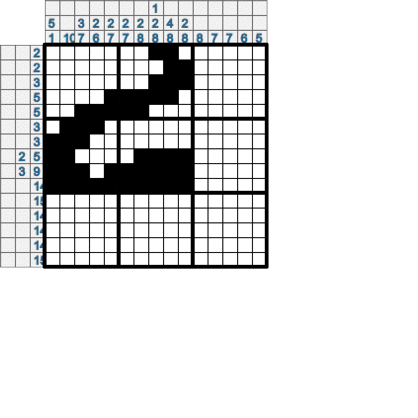
\includegraphics[width=5cm]{../Images/cat/cat3.png}
			\hspace{1cm}
          		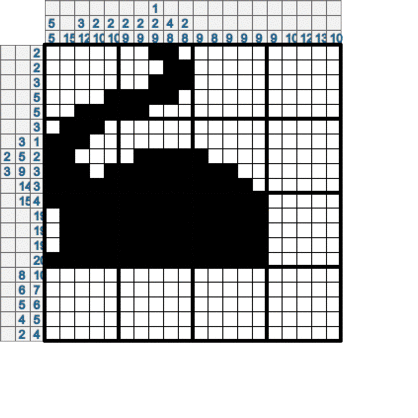
\includegraphics[width=5cm]{../Images/cat/cat4.png}
			\hspace{1cm}
          		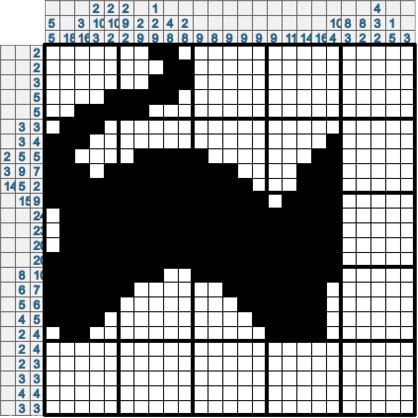
\includegraphics[width=5cm]{../Images/cat/cat5.png}
			\hspace{1cm}
			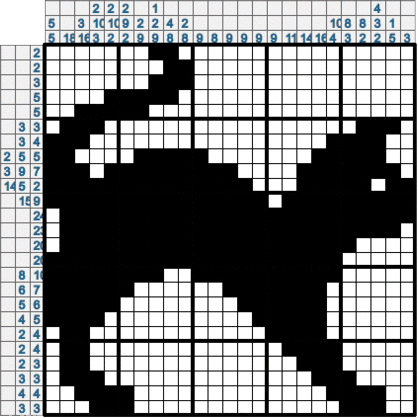
\includegraphics[width=5cm]{../Images/cat/cat6.png}
		\end{figure}
		
	
	\section{Maquettes de l'interface}
      
      		Ci-dessous les maquettes réalisées pour l'interface de notre application en français. Lorsque le joueur lance l'application, il tombe sur l'écran (1) lui demandant de rentrer son pseudo pour permettre à chaque joueur d'avoir son propre profil. S'il rentre un pseudo déjà existant, il charge son profil avec ses statistiques et ses chapitres débloqués sinon un nouveau profil est créer. L'utilisateur arrive ensuite sur la page d'accueil du logiciel (2) lui permettant de choisir parmi les différentes fonctionnalités. Le bouton \textit{Quitter} ferme l'application. Le bouton \textit{Options} renvoit sur la page d'options (3) qui permet à l'utilisateur de modifier ses préférences de jeu. Le bouton \textit{Règles}  permet d'afficher les règles générales du \textit{picross} (4). L'utilisateur peut voir ses statistiques et celles des autres utilisateurs en cliquant sur le bouton \textit{Classement}. Enfin, en cliquant sur le bouton \textit{Jouer}, l'utilisateur est envoyé sur la sélection du  chapitre (5) comportant tout les chapitres du jeu, didacticiel et mode évolutif inclus. Après avoir choisi un chapitre, il arrive sur la sélection de la grille (6) ainsi que le nombre d'étoiles obtenues sur les grilles déjà réussies. Lorsqu'il a choisi sa grille, la partie commence (7).
		
		
	\begin{figure}[H]
    		\begin{minipage}[c]{.46\linewidth}
       			\centering
       			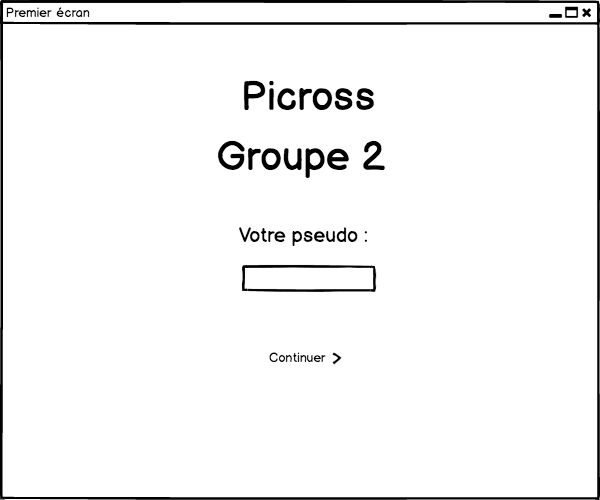
\includegraphics[width=8cm]{Maquettes/Premier_ecran.png}
        			\caption{(1) Ecran de connexion}
    		\end{minipage}
    		\hfill
   		\begin{minipage}[c]{.46\linewidth}
        			\centering
       			 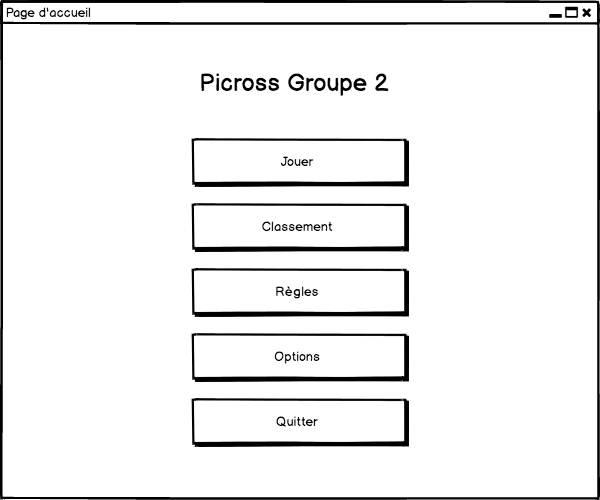
\includegraphics[width=8cm]{Maquettes/Page_Accueil.png}
        			\caption{(2) Page d'accueil}
    		\end{minipage}
	\end{figure}
	
	\begin{figure}[H]
    		\begin{minipage}[c]{.46\linewidth}
       			\centering
       			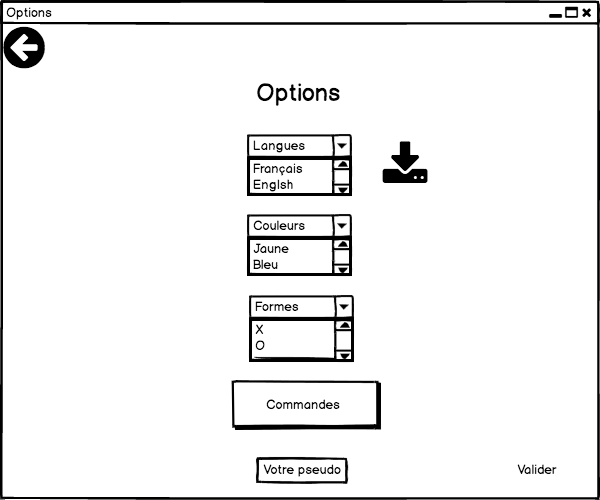
\includegraphics[width=8cm]{Maquettes/Options.png}
        			\caption{(3) Options}
    		\end{minipage}
    		\hfill
   		\begin{minipage}[c]{.46\linewidth}
        			\centering
       			 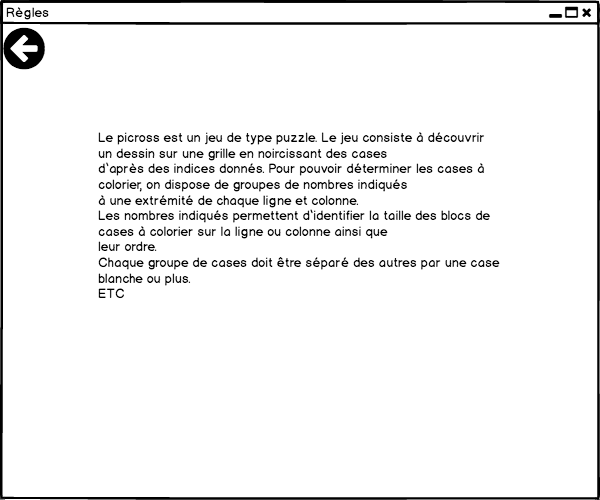
\includegraphics[width=8cm]{Maquettes/Regles.png}
        			\caption{(4) Règles}
    		\end{minipage}
	\end{figure}
	
	\begin{figure}[H]
    		\begin{minipage}[c]{.46\linewidth}
       			\centering
       			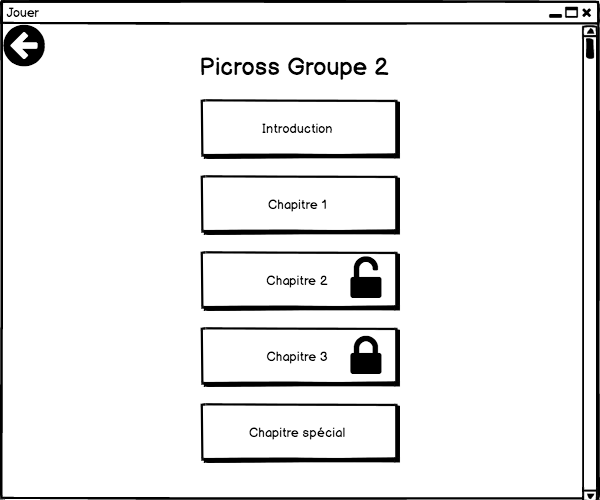
\includegraphics[width=8cm]{Maquettes/Jouer.png}
        			\caption{(5) Sélection du chapitre}
    		\end{minipage}
    		\hfill
   		\begin{minipage}[c]{.46\linewidth}
        			\centering
       			 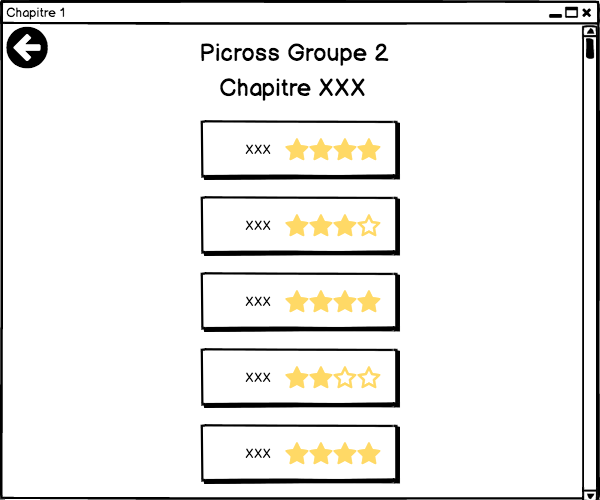
\includegraphics[width=8cm]{Maquettes/Chapitre_1.png}
        			\caption{Sélection de la grille}
    		\end{minipage}
	\end{figure}
	
	 \begin{figure}[H]
	 	\centering
		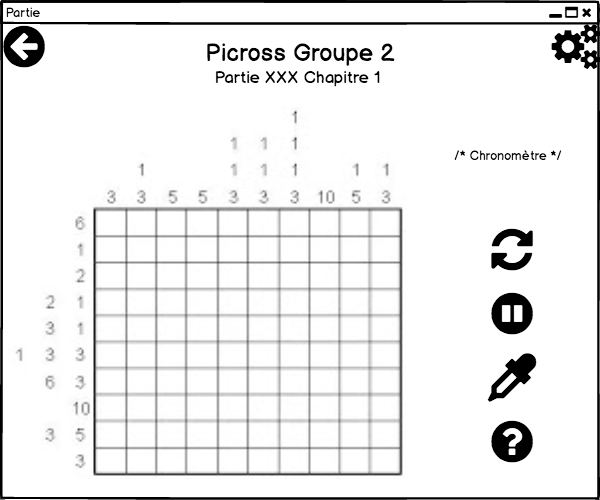
\includegraphics[width=8cm]{Maquettes/Partie.png}
		\caption{Partie}
    	\end{figure}


\end{document}
